\documentclass[10pt]{article}
\usepackage[letterpaper,textwidth=5.5in,textheight=9in,top=1in,headheight=12pt,headsep=25pt,footskip=30pt]{geometry}
\usepackage[T1]{fontenc}
\usepackage{mathptmx}
\usepackage{amsmath,amssymb}
\usepackage{graphicx}
\usepackage{booktabs}
\usepackage{multirow}
\usepackage{caption}
\usepackage{enumitem}
\usepackage[colorlinks=true,linkcolor=black,citecolor=blue,urlcolor=blue]{hyperref}
\captionsetup{font=small,labelfont=bf}
\setlength{\parindent}{0pt}
\setlength{\parskip}{5.5pt}
\setlist{itemsep=1pt,topsep=2pt}
\graphicspath{{../../}}
\newcommand{\rhoS}{$\rho$}

\begin{document}

\begin{center}
\rule{\textwidth}{4pt}\\[10pt]
{\LARGE\bfseries Where Does Heat Send People to the ER?\\[4pt] Predicting ZIP-Level Excess Heat Emergency Visits\\[2pt] in California and Los Angeles County}\\[8pt]
\rule{\textwidth}{1pt}\\[14pt]
\begin{tabular}{cc}
\textbf{Rohit Shetty} & \textbf{Utkarsh Landge}\\
University of Southern California & University of Southern California\\[8pt]
\textbf{Neel Kothari} & \textbf{Haochen (Char) Song}\\
University of Southern California & University of Southern California\\
\end{tabular}\\[6pt]
{\small CSCI 461: AI for Sustainable Development, Fall 2026 \quad Team HEATLA \quad Preliminary report}
\end{center}

\begin{center}\textbf{\large Abstract}\end{center}
\begin{quote}\small
Extreme heat sends more people to the emergency room (ER) in some neighborhoods than in others, and Los Angeles County has to decide where limited cooling resources go. We use UCLA Heat Maps estimates of heat-related excess ER visits for 1,675 California ZIP codes at four heat levels (2008--2018) as labels, and community data from CalEnviroScreen and the American Community Survey as inputs. We ask whether patterns learned elsewhere in California transfer to Los Angeles, whether added community features help within Los Angeles, and how predictions can feed a cooling-center siting model. A Poisson model trained outside Los Angeles ranks LA ZIPs on UCLA's level-4 label with Spearman \rhoS{} = 0.73 (R\textsuperscript{2} = 0.35), against 0.57 for the CalEnviroScreen index on the same ZIPs. On the excess from extreme-heat days alone, ranking holds (\rhoS{} = 0.68) but the size of the excess does not transfer (R\textsuperscript{2} = 0.09). Much of this skill comes from two inputs built from the same hospital records as the label: without them, extreme-heat ranking in LA is no better than the index. Within LA, four added community features raise Poisson \rhoS{} from 0.72 to 0.78. We also correct a missing-value error in the inputs, document how the labels are built, and state the siting problem as an integer program.
\end{quote}

\section{Introduction}

\subsection{Motivation}
Heat is a growing public-health hazard in California, and its effects are uneven. During the 2006 California heat wave, ER visits rose most for young children and older adults \cite{knowlton2009}, and within Los Angeles County communities with more outdoor workers had more heat-related ER visits \cite{riley2018}. The county runs cooling centers during heat events, but staff, hours and buildings are limited. Knowing which neighborhoods carry the most heat-related ER burden is a direct input to where those resources go. The work serves UN Sustainable Development Goals 3 (good health), 11 (sustainable cities) and 13 (climate action).

\subsection{Problem statement}
UCLA Heat Maps publishes, for every California ZIP code, an estimate of heat-related excess ER visits per 10,000 residents over 2008--2018 at four CalHeatScore heat levels. We treat these as labels and ask:
\begin{enumerate}
\item \textbf{Geographic transfer.} Can a model trained on community characteristics elsewhere in California predict which LA ZIPs carry the most heat-related ER burden, especially under extreme heat?
\item \textbf{Added community features.} Within LA, do four additional indicators (renters, households without a vehicle, uninsured residents, construction workers) improve prediction?
\item \textbf{Decision.} How should predicted burden be used to choose cooling centers, and does the prediction change that choice?
\end{enumerate}

\subsection{Outline of goals and approach}
The prediction tasks are regression on ZIP-level rates. We train Poisson regression, random forest and gradient boosting, evaluate them with spatial cross-validation and a hold-out of all of LA County, and compare against a training-mean baseline and the existing CalEnviroScreen index. Because UCLA's level-4 value turns out to total all heat levels, we also model the excess from level-4 days alone. Predictions then weight a maximal covering location problem that chooses which cooling centers to open. Section~\ref{sec:data} describes the data and preprocessing, Section~\ref{sec:results} the tasks and first results, and Section~\ref{sec:remaining} the remaining work.

\section{Related work}
\label{sec:related}

\textbf{Heat and emergency care in California.} Knowlton et al.\ \cite{knowlton2009} measured hospitalizations and ER visits during the 2006 California heat wave and found increases for heat illness, renal failure and cardiovascular causes, with the youngest and oldest at greatest risk. Basu et al.\ \cite{basu2012} linked apparent temperature to ER visits across California climate zones and tested confounding by air pollutants. Riley et al.\ \cite{riley2018}, the study UCLA's Heat Maps cite, used community-level data from LA County to show that ZIPs with more outdoor workers had higher heat-related ER rates. These works estimate associations at fixed locations; we test whether such relationships predict burden in a region the model has not seen.

\textbf{Community vulnerability indices.} Reid et al.\ \cite{reid2009} built a heat-vulnerability index from census and land-cover variables, and Gronlund \cite{gronlund2014} reviewed racial and socioeconomic disparities in heat-health effects. Derakhshan et al.\ \cite{derakhshan2024} are closest to our question: they asked whether social vulnerability indices correlate with excess heat ER outcomes in California and LA County and found that index choice matters. We use the CalEnviroScreen percentile as such an index baseline and ask whether a learned model ranks ZIPs better. Uejio et al.\ \cite{uejio2011} linked linguistic and social isolation to heat distress calls in Phoenix.

\textbf{Health conditions, pollution and access.} Heat raises emergency respiratory hospitalizations \cite{anderson2013} and childhood asthma ED admissions \cite{xu2013}, and air pollutants modify heat effects \cite{analitis2014}. Insurance status relates to how heat illness is treated in EDs \cite{hess2014}, and renters are less likely to have air conditioning \cite{scott2025}. These motivate our inputs (Table~\ref{tab:features}).

\textbf{Methods.} Spatially structured data make random cross-validation optimistic, because neighboring observations are near copies; Roberts et al.\ \cite{roberts2017} recommend blocked cross-validation, which we use. For siting we use the maximal covering location problem of Church and ReVelle \cite{church1974}.

\section{Data}
\label{sec:data}

\subsection{Description and sources}
The unit of observation is a ZIP code at one heat level. Table~\ref{tab:sources} lists the sources; all are public.

\begin{table}[!htbp]
\centering\small
\caption{Data sources.}
\label{tab:sources}
\begin{tabular}{@{}p{3.1cm}p{5.6cm}p{3.6cm}@{}}
\toprule
Source & What we use & Raw size \\
\midrule
UCLA Heat Maps (\texttt{zip\_ER} layer) & Label: excess ER visits per 10,000, 2008--2018, heat levels 1--4; population; heat days & 1,686 ZIPs $\times$ 4 levels = 6,744 rows \\
CalEnviroScreen 4.0 (OEHHA) & 10 tract inputs: PM2.5, ozone, asthma and heart-attack ED rates, poverty, age 65+, education, linguistic isolation, unemployment, housing burden; overall percentile (baseline) & 8,035 tracts \\
CalEnviroScreen 3.0 & Same 10 inputs from 2009--2015 (sensitivity check) & 8,035 tracts \\
ACS 2014--2018 5-year (Census API) & Renters, no vehicle, uninsured, construction workers & 33,120 ZCTAs \\
Census Gazetteer 2023 & ZIP centroid and land area & 33,791 ZCTAs \\
LA County cooling centers (2022) & Candidate sites for siting & 153 sites \\
\bottomrule
\end{tabular}
\end{table}

\subsection{What the label is}
We read UCLA's methods documentation \cite{ucla2025} and checked the published data. Three facts shape the project:
\begin{itemize}
\item \textbf{It is a model estimate, not a count.} UCLA fits a Bayesian spatial Poisson model to daily ER visits and temperature; excess visits are observed visits minus those expected at a typical temperature. Under UCLA's default setting, no socioeconomic inputs enter that model, so our features are not used to build the label.
\item \textbf{It is a total over eleven warm seasons} (May--October 2008--2018). UCLA's yearly values sum to it.
\item \textbf{It is cumulative across heat levels.} In all 1,675 ZIPs the level-4 row covers exactly 2,024 days, every warm-season day (184 $\times$ 11), and both day counts and labels rise with level. The level-$k$ value therefore covers all days at or below level $k$. This is our inference; UCLA does not state it. The excess on level-4 days alone is label(4) $-$ label(3), which we call the \emph{level-4-only} target.
\end{itemize}

\subsection{Preprocessing}
\textbf{Fusion.} CalEnviroScreen values are tract-level; we aggregate them to ZIPs as population-weighted means using each tract's ZIP field. ACS values are joined to ZIPs by ZCTA code. Population density is UCLA's population divided by Gazetteer land area.

\textbf{Missing-value correction.} CalEnviroScreen marks a missing tract value as $-999$. The first version of the pipeline averaged these markers into ZIP values, which produced impossible numbers (one ZIP had $-314.8$\% without a high-school degree) and changed the inputs of 436 of 1,675 ZIPs (92 of 287 in LA). We now set $-999$ to missing for each field before aggregation; no negative values remain. All results below use the corrected inputs.

\textbf{Cleaning and imputation.} We drop rows without a label, centroid or population (11 ZIPs). Rows with missing inputs are kept: 337 ZIPs have no CalEnviroScreen tract at all and 57 lack some inputs, so 394 of 1,675 (17 of 287 in LA) have at least one input filled with the training-fold median. Imputation and scaling are fitted on training data only.

\textbf{Data years.} The label covers 2008--2018. CalEnviroScreen 4.0 inputs describe about 2013--2019 and the added ACS features 2014--2018. UCLA's population is from the 2020 Census; it is also the label's denominator. Rerunning the models with 2010 Census population (for density, and for density plus the Poisson weight) moved level-4 rank correlation by at most 0.02 in either direction, well inside the bootstrap intervals, so we keep the 2020 values.

\textbf{Removed inputs.} Total population is not an input (density is). Two inputs, the asthma and heart-attack ED rates, come from the same state ER records as the label; we keep them but test removing them (Section~\ref{sec:ablation}).

\subsection{Processed dataset}
After cleaning the statewide table has 1,675 ZIPs and 6,700 rows; LA County has 287 ZIPs (1,148 rows). The LA-only experiments use the 287 LA ZIPs at level 4. Table~\ref{tab:features} lists the inputs and Table~\ref{tab:label} the label by level. Labels are continuous rates, so there is no class balance to report; instead Figure~\ref{fig:label} shows their distribution by level.

\begin{table}[!htbp]
\centering\small
\caption{Model inputs. ``All'' = the statewide model and both LA configurations. CES = CalEnviroScreen.}
\label{tab:features}
\resizebox{\textwidth}{!}{%
\begin{tabular}{@{}llllll@{}}
\toprule
Input & Definition & Period & Source & Used in & Evidence \\
\midrule
Heat level & CalHeatScore level 1--4 & 2008--18 & UCLA & Statewide & -- \\
PM2.5, ozone & Annual mean; mean 8-hr max & 2015--19 & CES 4.0 & All & \cite{analitis2014,basu2012} \\
Asthma, heart-attack ED & Age-adjusted visits per 10,000 & 2015--17 & CES 4.0 & All & \cite{xu2013,anderson2013,knowlton2009} \\
Poverty & \% below 2$\times$ federal poverty level & 2015--19 & CES 4.0 & All & \cite{reid2009,gronlund2014} \\
Age 65+, education & \% 65+; \% over 25 without high school & 2015--19 & CES 4.0 & All & \cite{reid2009,knowlton2009} \\
Ling.\ isolation, unemployment & \% limited-English households; \% unemployed & 2015--19 & CES 4.0 & All & \cite{uejio2011,gronlund2014} \\
Housing burden & \% low-income paying $>$50\% on housing & 2013--17 & CES 4.0 & All & \cite{gronlund2014} \\
Population density & Persons per sq.\ mile & 2020 & UCLA, Census & All & \cite{uejio2011} (indirect) \\
Renters, no vehicle & \% of occupied housing units & 2014--18 & ACS & LA augmented & \cite{scott2025,derakhshan2024} \\
Uninsured, construction & \% population; \% employed residents & 2014--18 & ACS & LA augmented & \cite{hess2014,riley2018} \\
\bottomrule
\end{tabular}}
\end{table}

\begin{table}[!htbp]
\centering\small
\caption{Label by heat level: excess ER visits per 10,000, total over May--October 2008--2018.}
\label{tab:label}
\begin{tabular}{@{}llrrrrr@{}}
\toprule
& & \multicolumn{2}{c}{Published (cumulative)} & \multicolumn{2}{c}{That level alone} & Share of \\
Region & Level & Mean & SD & Mean & SD & level-4 total \\
\midrule
California (1,675 ZIPs) & 1 & 2.08 & 0.73 & 2.08 & 0.73 & 15.1\% \\
 & 2 & 3.93 & 1.17 & 1.84 & 0.65 & 13.4\% \\
 & 3 & 6.84 & 1.94 & 2.92 & 1.22 & 21.2\% \\
 & 4 & 13.80 & 7.82 & 6.95 & 7.10 & 50.4\% \\
\midrule
Los Angeles (287 ZIPs) & 1 & 2.47 & 0.61 & 2.47 & 0.61 & 24.6\% \\
 & 2 & 4.40 & 1.09 & 1.92 & 0.59 & 19.2\% \\
 & 3 & 6.93 & 1.83 & 2.53 & 0.88 & 25.2\% \\
 & 4 & 10.04 & 3.10 & 3.11 & 1.68 & 30.9\% \\
\bottomrule
\end{tabular}
\end{table}

\begin{figure}[!htbp]
\centering
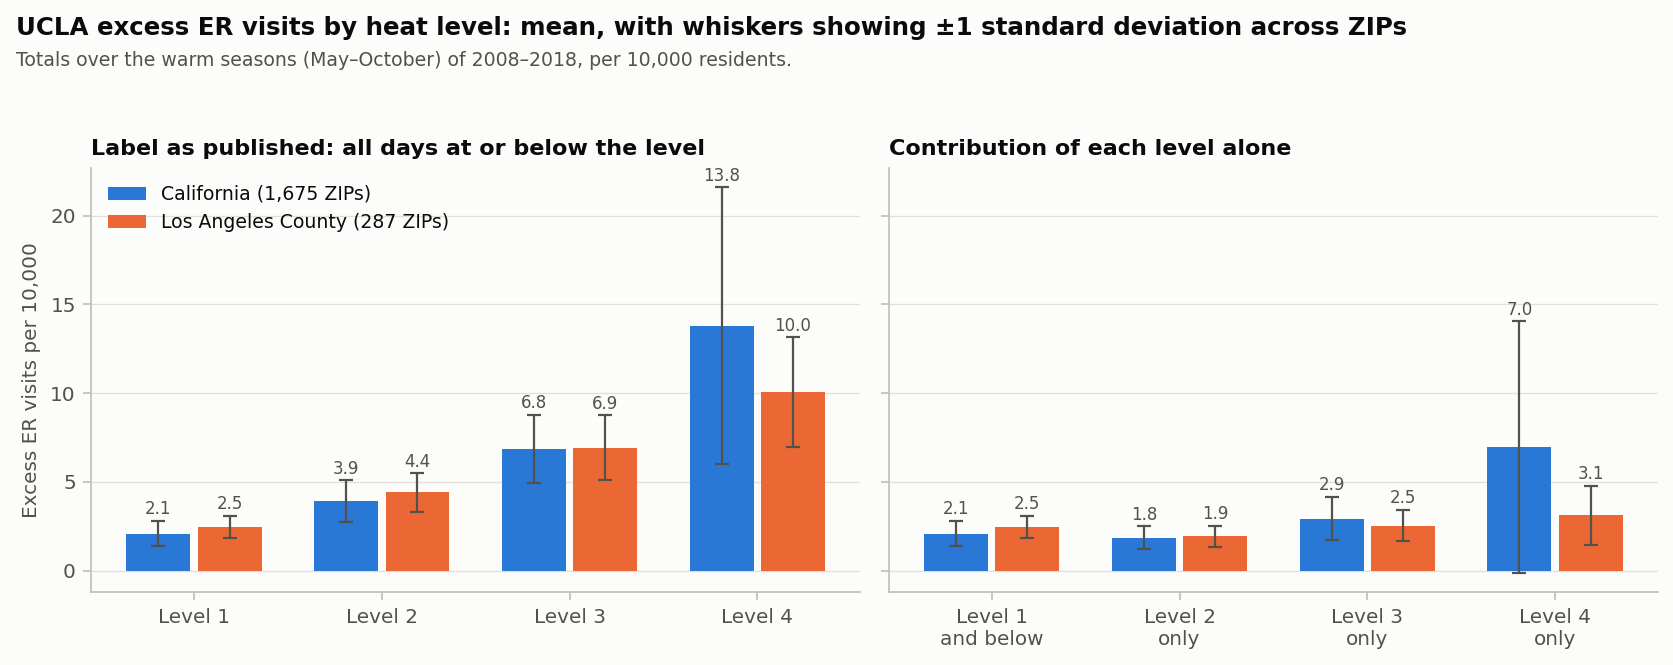
\includegraphics[width=\textwidth]{results/member3/label_eda/label_mean_sd_by_level.png}
\caption{Mean label by heat level with $\pm$1 SD across ZIPs. Left: as published. Right: each level's own days.}
\label{fig:label}
\end{figure}

\textbf{Exploratory findings.} Statewide, the mean doubles from level 3 to 4 and the spread quadruples; level-4 days alone account for half of the total. LA is different at level 4: its level-4-only mean is 3.11 against 7.75 for the rest of California. Levels also rank ZIPs differently: across California, the rank correlation between level-1 and level-4 labels is $-0.29$. Figure~\ref{fig:corr} shows Spearman correlations at level 4. The two ED-rate inputs correlate most with the label (0.52 and 0.50), followed by poverty (0.44) and unemployment (0.39); density correlates negatively ($-0.44$), so dense urban ZIPs have lower excess rates.

\begin{figure}[!htbp]
\centering
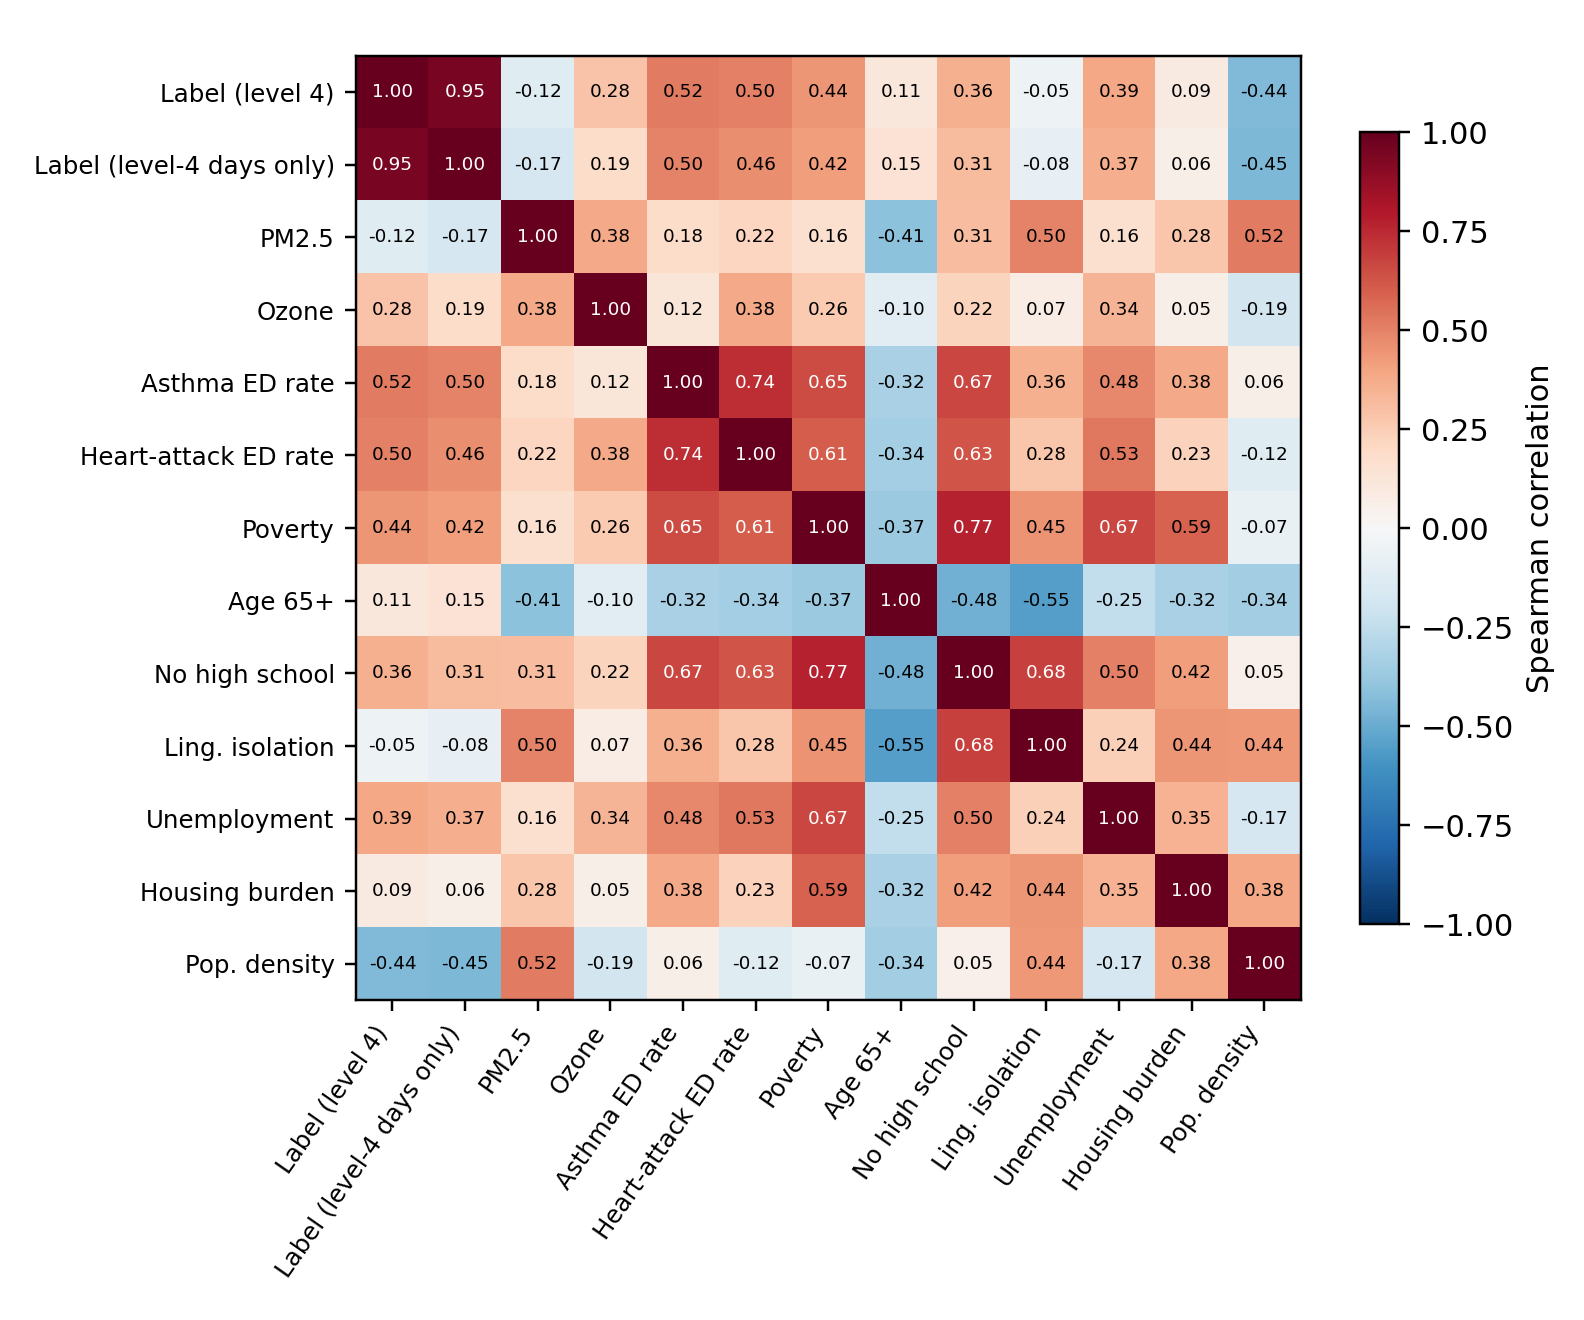
\includegraphics[width=0.78\textwidth]{reports/prelim/fig_corr.png}
\caption{Spearman correlation matrix, level 4, all California ZIPs (pairwise complete).}
\label{fig:corr}
\end{figure}

\section{Tasks, approach and first results}
\label{sec:results}

\subsection{Task and setup}
\textbf{Task.} Regression: given a ZIP's community inputs (and heat level, in statewide models), predict UCLA's excess ER visits per 10,000. Two targets: the published level-$k$ label and the level-$k$-only excess. Predictions are used to rank ZIPs and, downstream, to weight the siting model.

\textbf{Models.} Poisson regression with a log link (ridge penalty 1.0, population-weighted, standardized inputs), suited to non-negative rates; random forest (500 trees, minimum leaf 2); gradient boosting (scikit-learn defaults). Seed 42. \textbf{Baselines:} the training-fold mean, and the CalEnviroScreen 4.0 percentile, an existing index, compared on rank only and on the same ZIPs.

\textbf{Evaluation.} Table~\ref{tab:setups} gives the three designs. Folds are $k$-means clusters of ZIP centroids, so neighboring ZIPs are tested together \cite{roberts2017}, and all four heat-level rows of a ZIP stay in one fold. Metrics: R\textsuperscript{2}, Spearman \rhoS{}, and top-10\% recall (the share of the truly highest-burden 10\% of ZIPs that a model also ranks in its top 10\%). Error = prediction $-$ label.

\begin{table}[!htbp]
\centering\small
\caption{Experimental designs.}
\label{tab:setups}
\begin{tabular}{@{}p{2.3cm}p{3.4cm}p{3.4cm}p{3.4cm}@{}}
\toprule
& A. Statewide spatial CV & B. LA hold-out & C. LA-only spatial CV \\
\midrule
Question & Out-of-area skill & Transfer to LA & Added features in LA \\
Train & 9 of 10 folds & California outside LA: 1,388 ZIPs, 5,552 rows & 4 of 5 LA folds \\
Test & Held-out fold (1,675 ZIPs, 6,700 rows) & LA: 287 ZIPs, 1,148 rows & Held-out LA fold (287 ZIPs) \\
Heat levels & 1--4 & 1--4 & 4 only \\
Inputs & 12 & 12 & 11 base / 15 augmented \\
\bottomrule
\end{tabular}
\end{table}

\begin{figure}[!htbp]
\centering
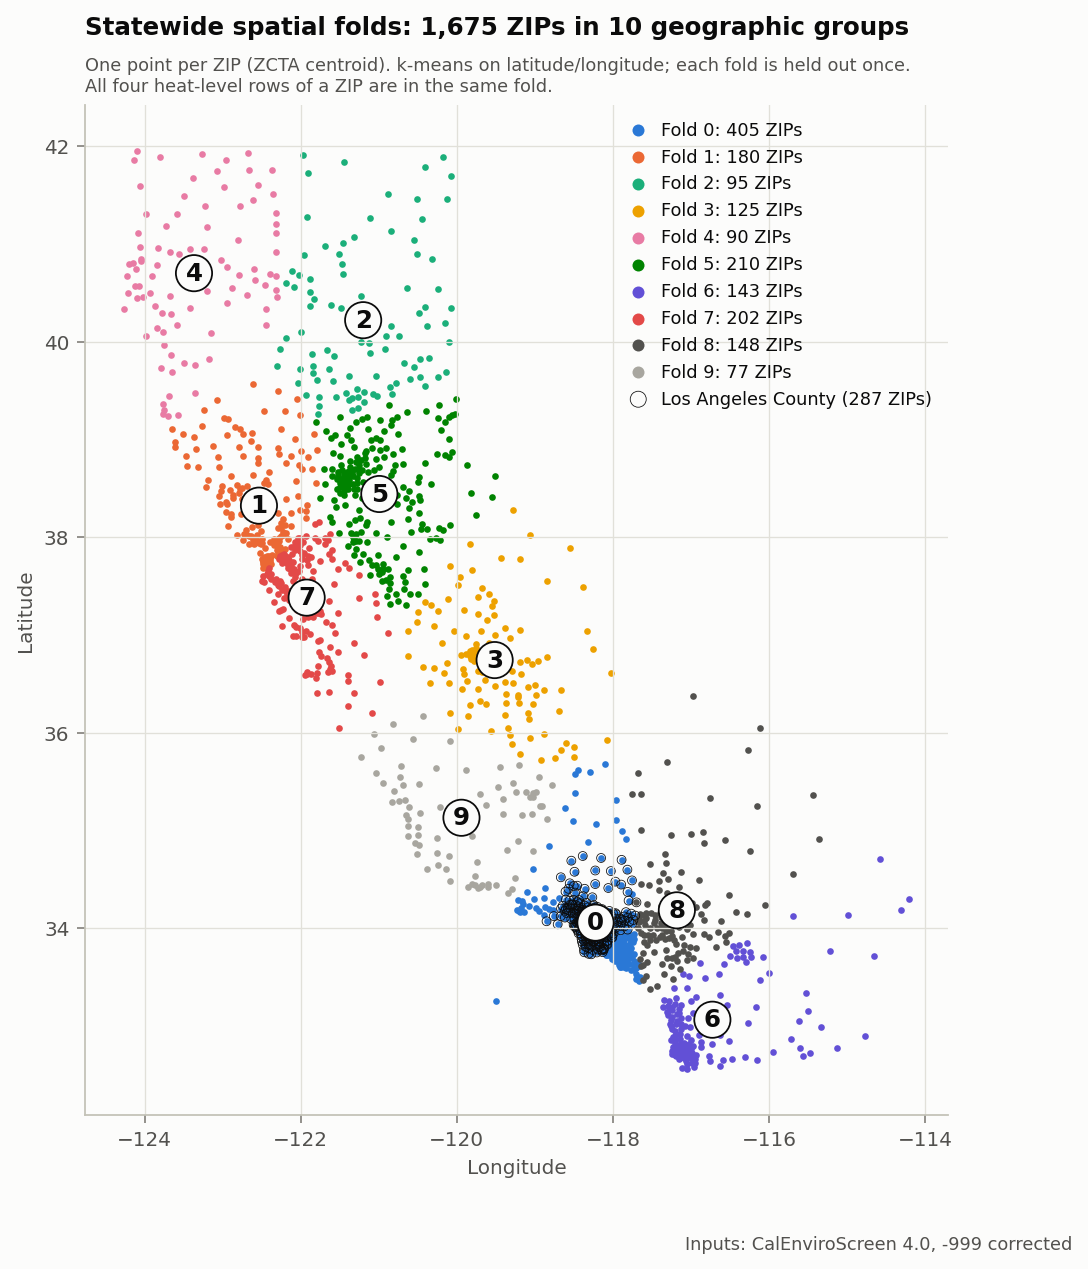
\includegraphics[width=0.62\textwidth]{results/member1/ces40_fixed/figures/fold_map_statewide.png}
\caption{The ten statewide folds (design A). 286 of the 287 LA ZIPs fall in one fold, so for LA designs A and B are nearly the same test.}
\label{fig:folds}
\end{figure}

\subsection{Pooled scores hide weak within-level skill}
Table~\ref{tab:levels} shows the LA hold-out. Pooled over levels, every model looks strong (\rhoS{} $\approx$ 0.9), but that mostly reflects the gap between levels, which the heat-level input gives away. Within a level, skill is much lower and rises with level. The tree models rank LA ZIPs well at level 4 but have negative R\textsuperscript{2}: they carry the higher level-4 values of the rest of California into LA.

\begin{table}[!htbp]
\centering\small
\caption{LA hold-out (design B), published label, models trained on all levels outside LA.}
\label{tab:levels}
\begin{tabular}{@{}lrrrrrrrrr@{}}
\toprule
& \multicolumn{3}{c}{Poisson} & \multicolumn{3}{c}{Random forest} & \multicolumn{3}{c}{Gradient boosting} \\
\cmidrule(lr){2-4}\cmidrule(lr){5-7}\cmidrule(lr){8-10}
Scope & R\textsuperscript{2} & \rhoS{} & Top-10 & R\textsuperscript{2} & \rhoS{} & Top-10 & R\textsuperscript{2} & \rhoS{} & Top-10 \\
\midrule
Pooled, levels 1--4 & 0.781 & 0.905 & 0.75 & 0.619 & 0.911 & 0.66 & 0.642 & 0.898 & 0.70 \\
Level 1 & $-$0.235 & 0.282 & 0.14 & $-$0.047 & 0.213 & 0.17 & $-$0.259 & 0.148 & 0.03 \\
Level 2 & 0.046 & 0.468 & 0.21 & 0.212 & 0.480 & 0.34 & $-$0.140 & 0.267 & 0.21 \\
Level 3 & 0.277 & 0.630 & 0.24 & 0.321 & 0.531 & 0.31 & 0.243 & 0.487 & 0.21 \\
Level 4 & 0.349 & 0.730 & 0.34 & $-$0.483 & 0.688 & 0.14 & $-$0.291 & 0.683 & 0.24 \\
\bottomrule
\end{tabular}
\end{table}

Because levels behave so differently, we also trained one model per heat level (without the heat-level input) and compared it with the all-level model on the same LA ZIPs (Table~\ref{tab:levelspec}). It did not help at level 4: it has a quarter of the training data, all from regions with higher level-4 values.

\begin{table}[!htbp]
\centering\small
\caption{LA hold-out, level 4: one model for all levels vs.\ a level-4-only model.}
\label{tab:levelspec}
\begin{tabular}{@{}lrrrrrr@{}}
\toprule
& \multicolumn{3}{c}{All-level model} & \multicolumn{3}{c}{Level-specific model} \\
\cmidrule(lr){2-4}\cmidrule(lr){5-7}
Model & R\textsuperscript{2} & \rhoS{} & Top-10 & R\textsuperscript{2} & \rhoS{} & Top-10 \\
\midrule
Poisson & 0.349 & 0.730 & 0.34 & 0.174 & 0.711 & 0.28 \\
Random forest & $-$0.483 & 0.688 & 0.14 & $-$0.485 & 0.683 & 0.14 \\
Gradient boosting & $-$0.291 & 0.683 & 0.24 & $-$0.325 & 0.670 & 0.24 \\
\bottomrule
\end{tabular}
\end{table}

\subsection{Extreme heat alone, and the CalEnviroScreen baseline}
On the level-4-only target, Poisson still ranks LA ZIPs well (\rhoS{} = 0.68) and top-10\% recall does not fall, but R\textsuperscript{2} drops to 0.09 (95\% bootstrap interval $-0.12$ to 0.24). Extreme-day excess averages 7.75 per 10,000 outside LA and 3.11 inside it, so the model can tell which LA ZIPs are worse but not by how much. Table~\ref{tab:ces} compares against the index on the 273 LA ZIPs that have a percentile.

\begin{table}[!htbp]
\centering\small
\caption{Level 4, matched ZIPs: models vs.\ CalEnviroScreen percentile (rank metrics).}
\label{tab:ces}
\begin{tabular}{@{}llrrrrr@{}}
\toprule
Design & Target & ZIPs & CES \rhoS{} & Poisson \rhoS{} & CES top-10 & Poisson top-10 \\
\midrule
B. LA hold-out & Published label & 273 & 0.566 & 0.757 & 0.15 & 0.30 \\
B. LA hold-out & Level-4 only & 273 & 0.498 & 0.707 & 0.15 & 0.37 \\
A. Statewide CV & Published label & 1,326 & 0.300 & 0.647 & 0.11 & 0.24 \\
A. Statewide CV & Level-4 only & 1,326 & 0.254 & 0.597 & 0.09 & 0.29 \\
\bottomrule
\end{tabular}
\end{table}

\subsection{Without the ER-rate inputs}
\label{sec:ablation}
Removing the asthma and heart-attack ED rates lowers level-4 rank correlation for every model in both designs. For Poisson on the LA hold-out, \rhoS{} falls from 0.730 to 0.633 on the published label and from 0.681 to 0.502 on the level-4-only target, where the index scores 0.498 on matched ZIPs. Prior ER use may genuinely mark vulnerable communities, so the inputs are not invalid, but the model's skill under extreme heat rests heavily on them.

\subsection{Sensitivity to input year}
Rerunning everything on CalEnviroScreen 3.0, whose inputs describe 2009--2015 (inside the label period), changed level-4 results by less than their confidence intervals (LA hold-out Poisson \rhoS{} 0.744 vs 0.730). The mismatch between input and label years has a small measured effect.

\subsection{Added community features within LA}
Design C compares 11 base inputs with the same inputs plus the four ACS features, on identical ZIPs and folds (Table~\ref{tab:part2}, Figure~\ref{fig:part2}). The four features raise R\textsuperscript{2} and \rhoS{} for every model, most for Poisson, whose error falls in all five folds; top-10\% recall does not improve. The gain applies to the published label: on the level-4-only target the features no longer help (Poisson \rhoS{} 0.637 $\to$ 0.648). Without the ER-rate inputs they help more (0.553 $\to$ 0.691), but on level-4 days alone no model then beats the index (augmented Poisson 0.432 vs 0.498). Designs B and C differ in training region, levels and inputs, so their numbers are not directly comparable.

\begin{table}[!htbp]
\centering\small
\caption{LA-only spatial CV (design C), level 4, 287 ZIPs.}
\label{tab:part2}
\begin{tabular}{@{}lrrrrrr@{}}
\toprule
& \multicolumn{3}{c}{Base (11 inputs)} & \multicolumn{3}{c}{Augmented (15 inputs)} \\
\cmidrule(lr){2-4}\cmidrule(lr){5-7}
Model & R\textsuperscript{2} & \rhoS{} & Top-10 & R\textsuperscript{2} & \rhoS{} & Top-10 \\
\midrule
Poisson & 0.403 & 0.718 & 0.34 & 0.483 & 0.780 & 0.34 \\
Random forest & 0.421 & 0.685 & 0.17 & 0.460 & 0.710 & 0.21 \\
Gradient boosting & 0.425 & 0.718 & 0.31 & 0.468 & 0.731 & 0.28 \\
Training-fold mean & $-$0.111 & -- & -- & & & \\
\bottomrule
\end{tabular}
\end{table}

\begin{figure}[!htbp]
\centering
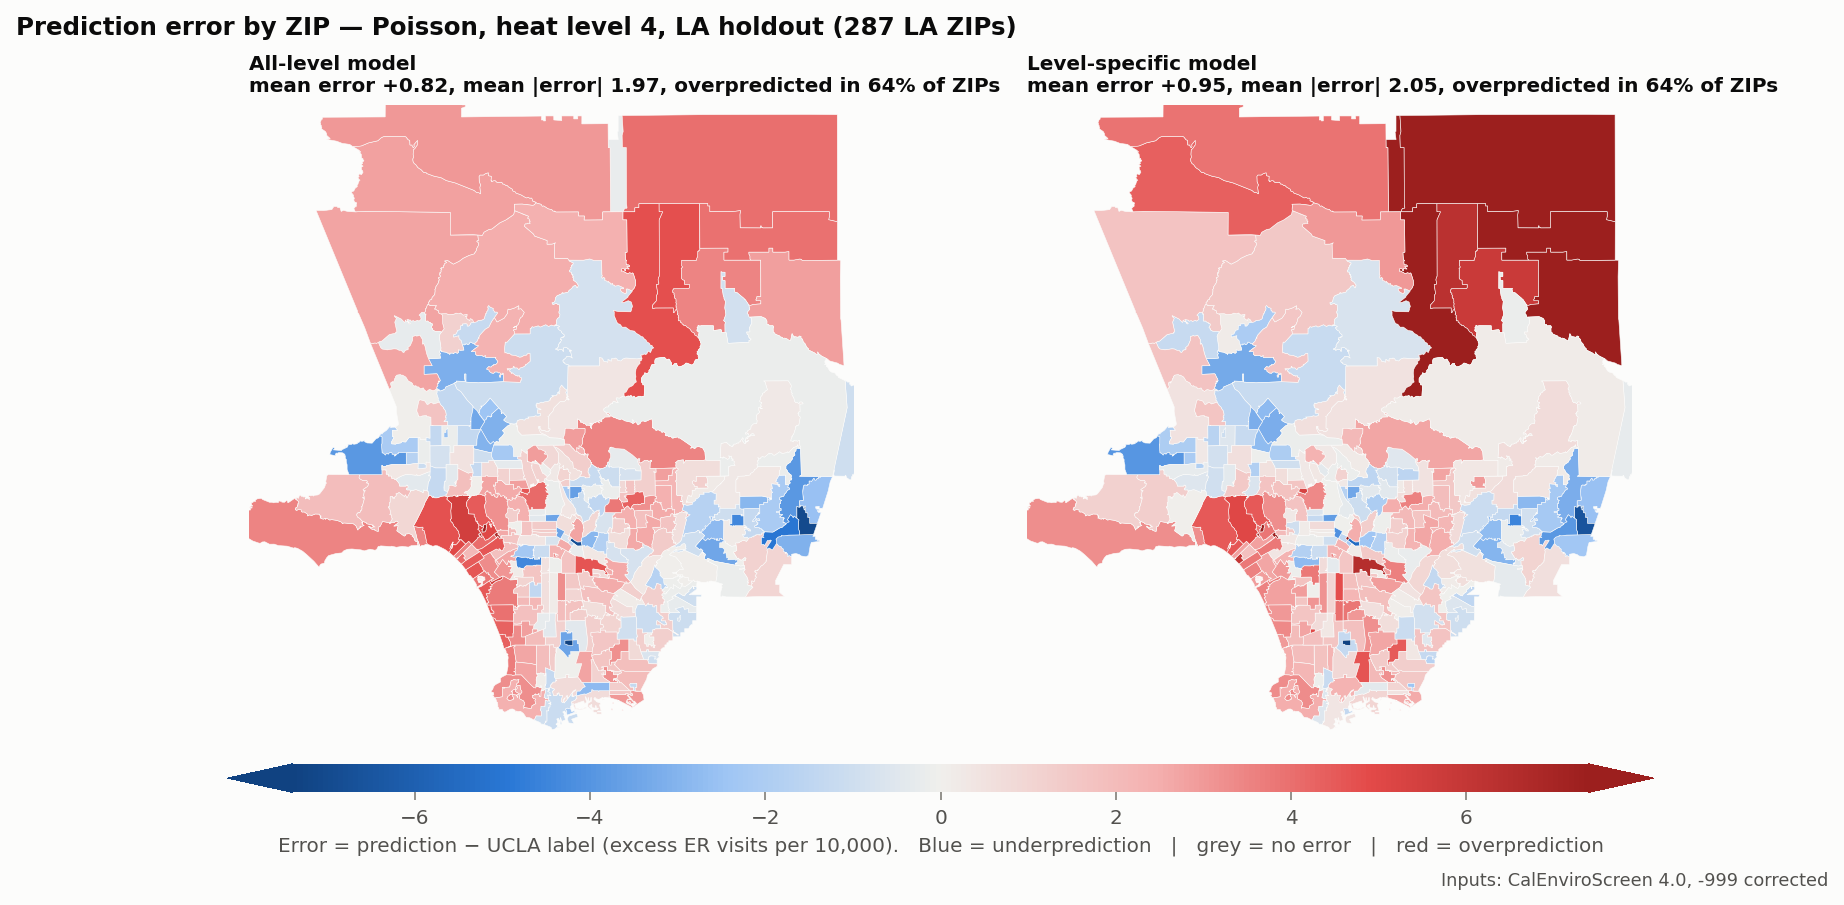
\includegraphics[width=\textwidth]{results/member1/ces40_fixed/figures/map_la_holdout_L4_poisson_error.png}
\caption{Where the errors are: prediction $-$ label, LA hold-out, level 4, Poisson. Red = overprediction.}
\label{fig:errors}
\end{figure}

\textbf{Where the errors are.} Poisson predictions are compressed (SD 1.75 against 3.10 for the labels), so low-burden ZIPs are overpredicted and high-burden ZIPs underpredicted (Figure~\ref{fig:errors}). Overprediction is largest on the Westside and South Bay coast; the inland San Fernando and San Gabriel Valleys are underpredicted.

\begin{figure}[!htbp]
\centering
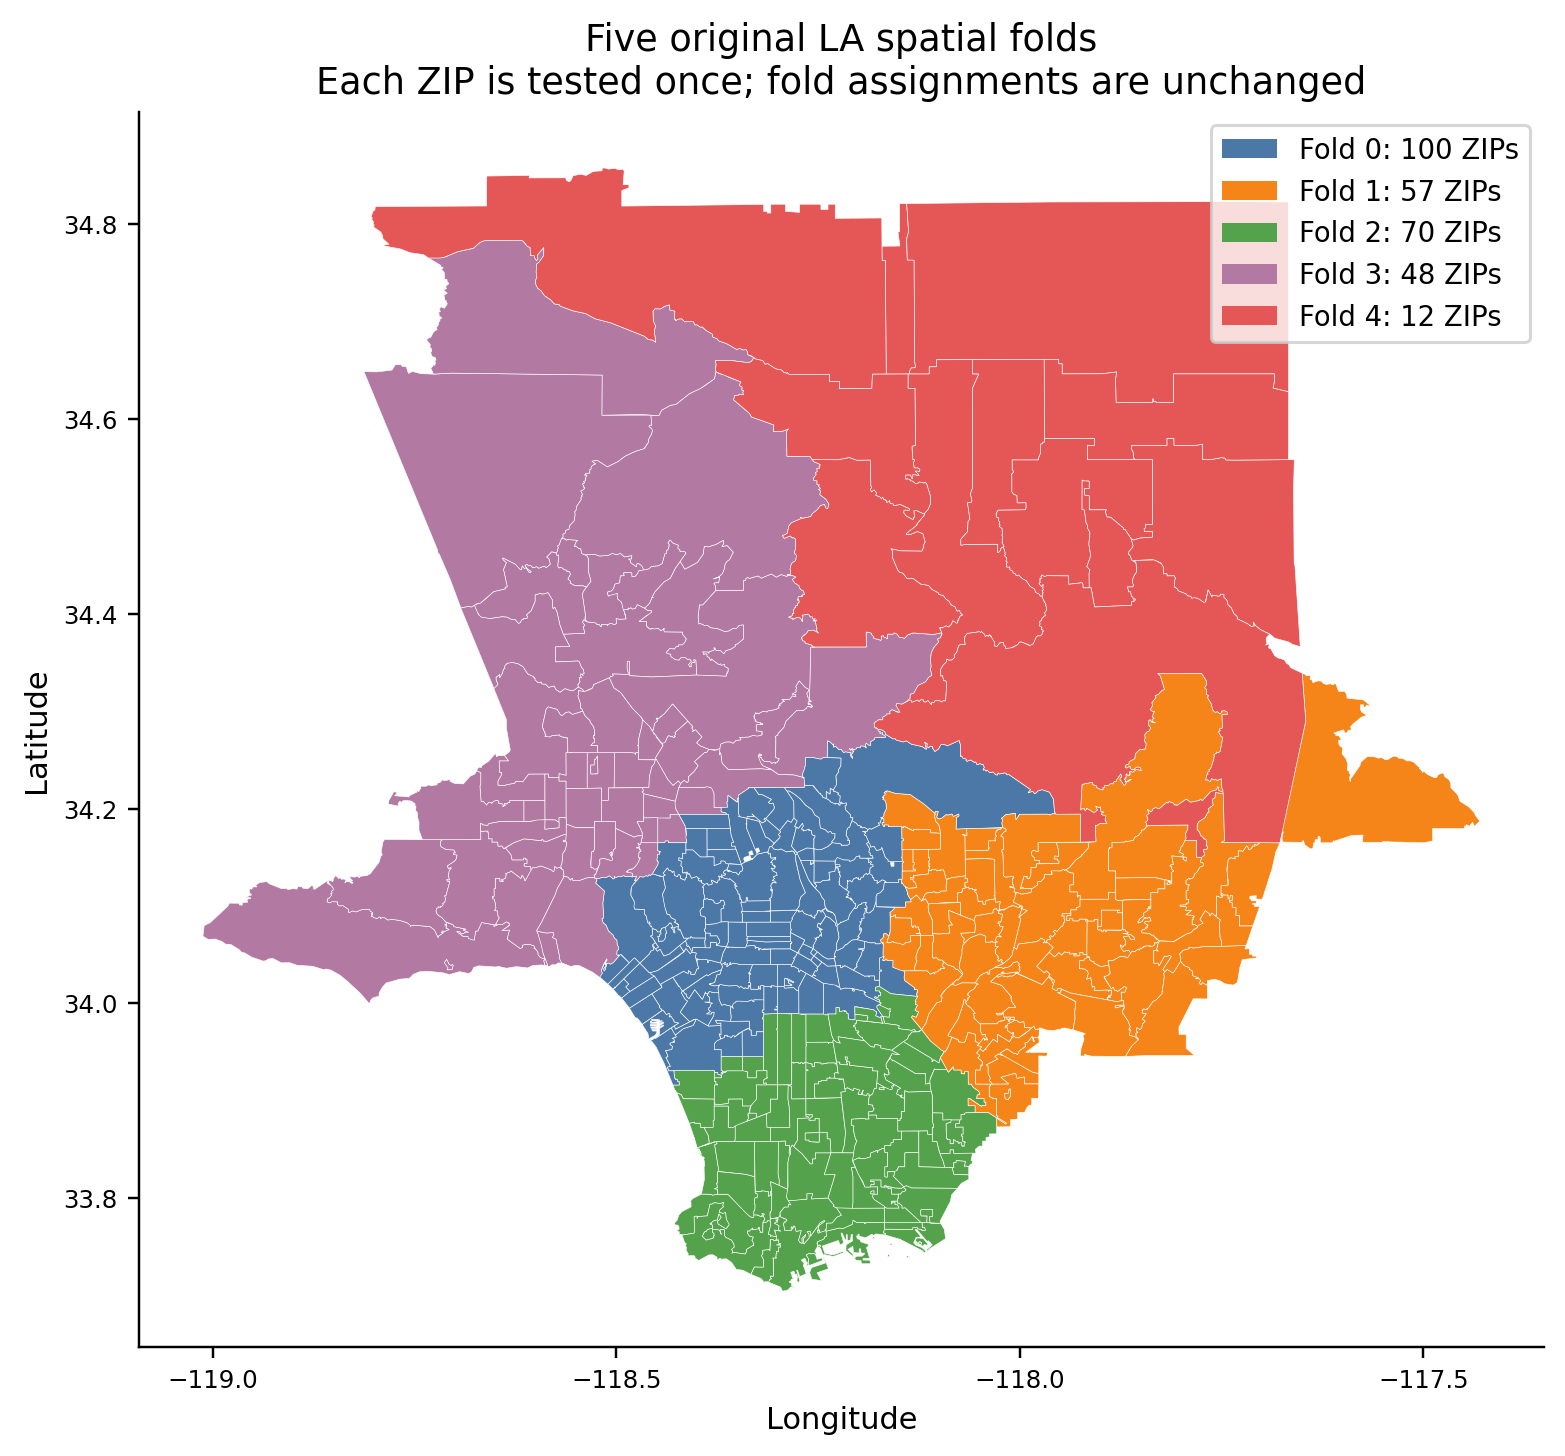
\includegraphics[width=0.55\textwidth]{part2/results/feature_comparison/figures/LA_spatial_folds.png}
\caption{The five LA spatial folds used in design C (100, 57, 70, 48 and 12 ZIPs).}
\label{fig:lafolds}
\end{figure}

\begin{figure}[!htbp]
\centering
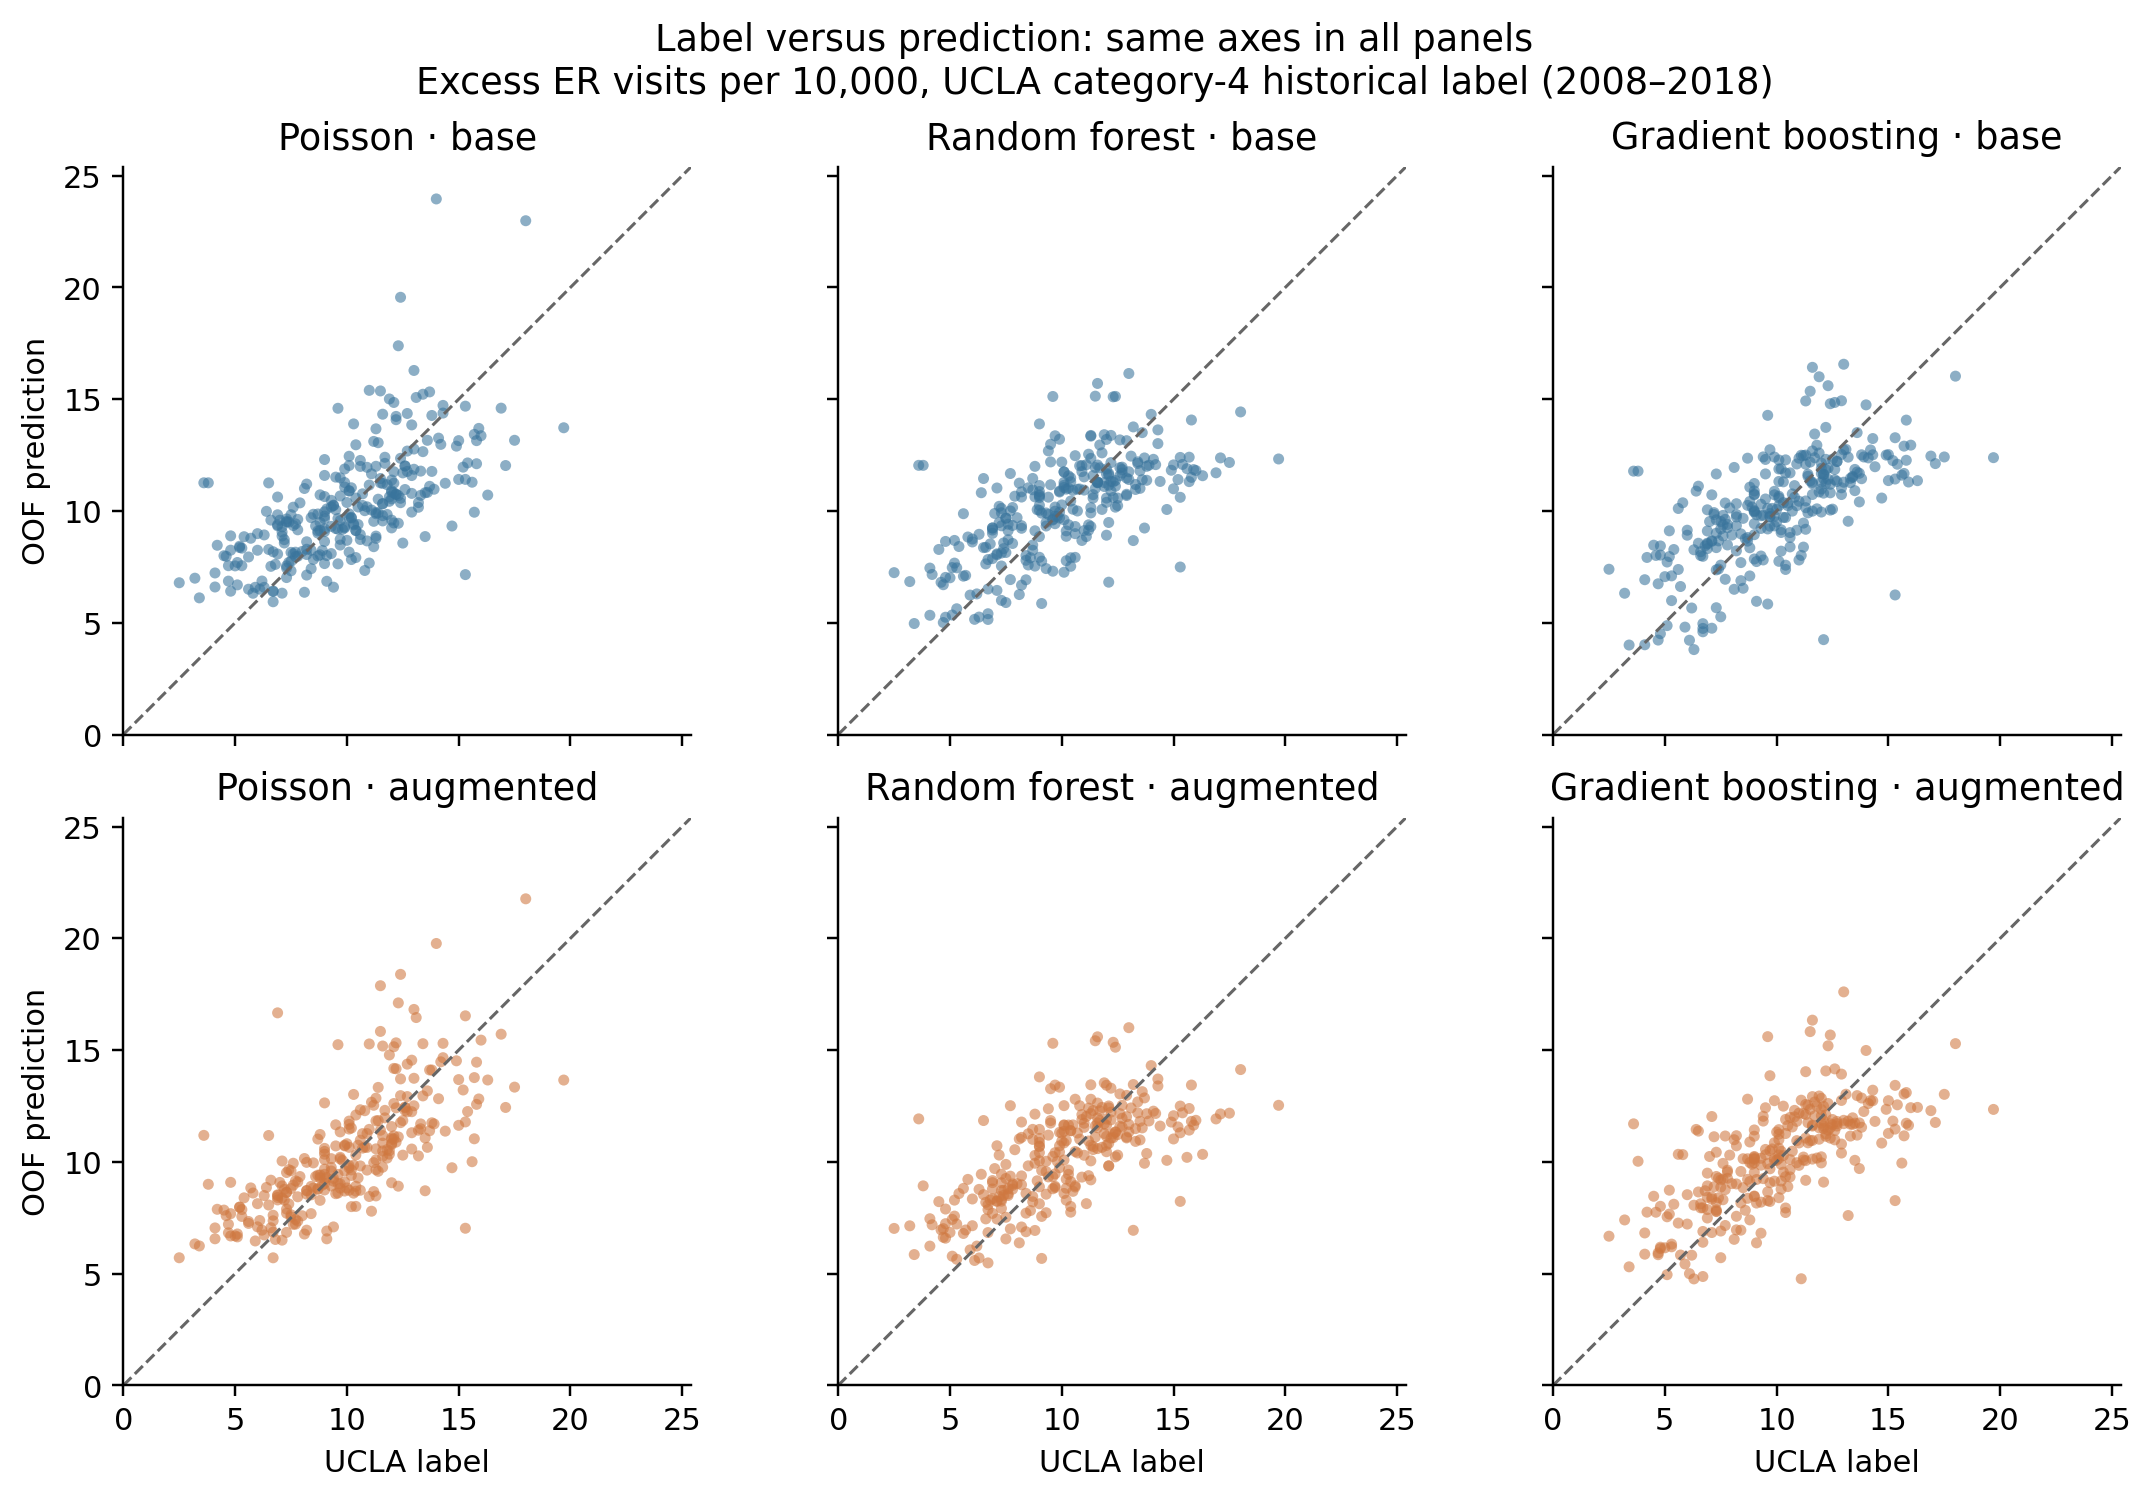
\includegraphics[width=0.85\textwidth]{part2/results/feature_comparison/figures/label_vs_prediction.png}
\caption{UCLA label vs.\ out-of-fold prediction, design C. Points above the dashed line are overpredicted.}
\label{fig:scatter}
\end{figure}

\begin{figure}[!htbp]
\centering
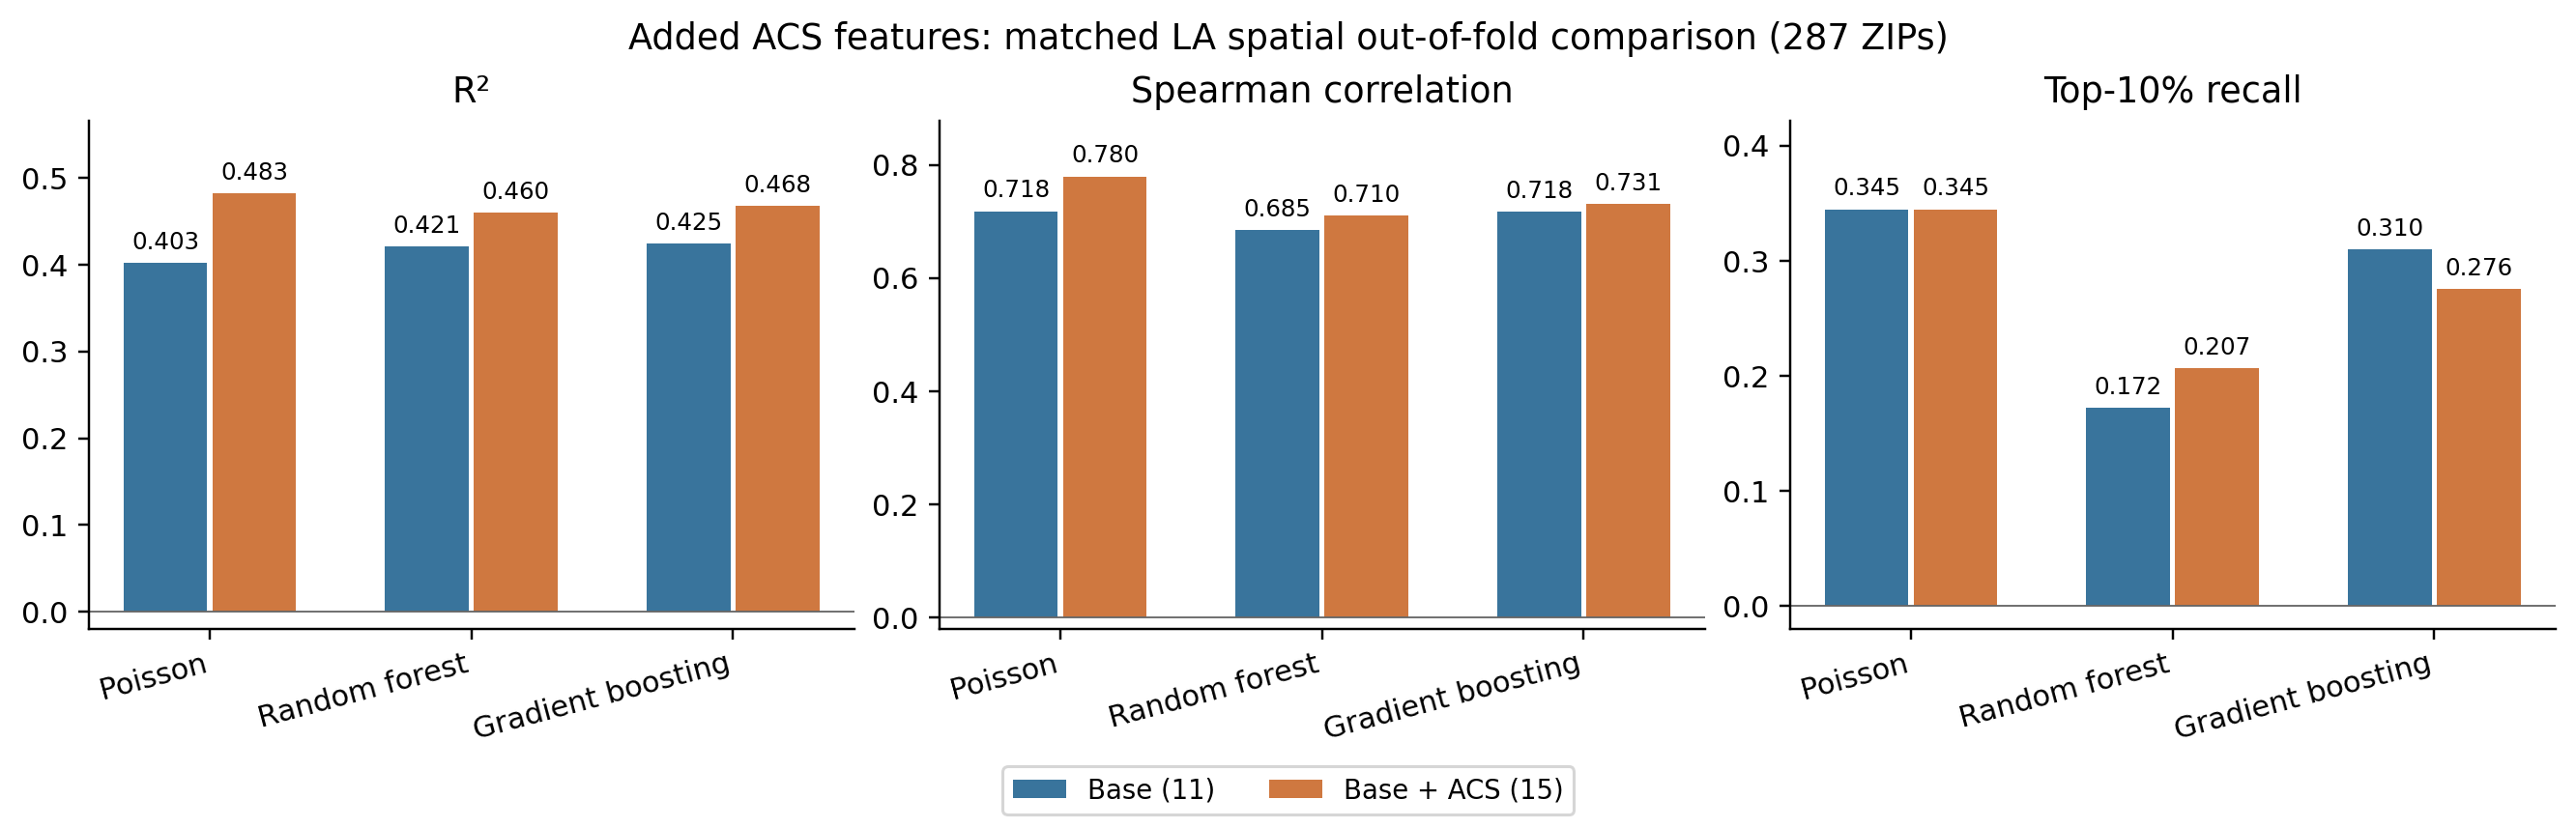
\includegraphics[width=\textwidth]{part2/results/feature_comparison/figures/model_comparison.png}
\caption{Base vs.\ augmented inputs, LA-only spatial CV (design C).}
\label{fig:part2}
\end{figure}

\subsection{Downstream task: cooling-center siting}
Predictions become the weights of a maximal covering location problem \cite{church1974}. Let $Z$ be the 287 LA ZIPs (centroids), $S$ the 153 county cooling centers, $w_z = \max(0,\hat r_z)\,p_z/10{,}000$ the predicted excess visits in ZIP $z$ ($\hat r_z$ predicted rate, $p_z$ population), $a_{zs}=1$ if the center is within radius $R$, and $k$ the number of centers. With $x_s$ selecting centers and $y_z$ marking covered ZIPs:
\[
\max \sum_{z\in Z} w_z y_z \quad\text{s.t.}\quad y_z \le \sum_{s\in S} a_{zs}x_s\;\;\forall z,\qquad \sum_{s\in S} x_s \le k,\qquad x_s, y_z\in\{0,1\}.
\]
A ZIP counts once however many centers reach it. We solve it exactly with CBC and compare with a greedy heuristic; the exact solution is never worse (largest gap 3.9 points). Weights come from the design-C augmented Poisson out-of-fold predictions.

\textbf{Does the prediction change the decision?} We score every plan on the true UCLA-label burden and compare plans chosen with model predictions, with the label itself (perfect information), with population alone, and at random (Table~\ref{tab:siting}). Prediction-based plans come within 0.25 points of perfect information on average over 16 radius and budget settings, and beat random selection by 17.5 points. But they beat population-only plans by just 0.8 points: most of the gain comes from where people live, and in LA, where every ZIP already has a label, the model adds little to this decision. Its value is where labels do not exist, such as the tract level (next section) or other regions. Adding 149 county libraries as candidate sites raises the share of burden reachable within 2 miles from 69\% to 88\%.

\begin{table}[!htbp]
\centering\small
\caption{Share of true (UCLA-label) burden within 2 miles of the chosen sites.}
\label{tab:siting}
\begin{tabular}{@{}lrrrr@{}}
\toprule
Plan (existing 153 centers) & $k=5$ & $k=10$ & $k=20$ & $k=40$ \\
\midrule
Model predictions & 13.0\% & 22.0\% & 35.2\% & 53.4\% \\
UCLA label (perfect information) & 13.2\% & 22.0\% & 35.7\% & 54.2\% \\
Population only & 12.3\% & 20.8\% & 33.9\% & 52.8\% \\
Random (mean of 100) & 5.3\% & 9.8\% & 17.9\% & 31.8\% \\
\midrule
Model predictions, centers + libraries & 13.2\% & 23.2\% & 40.0\% & 61.3\% \\
\bottomrule
\end{tabular}
\end{table}

\subsection{Downstream task: from ZIPs to census tracts}
A ZIP can hold very different neighborhoods, so we split each LA ZIP's UCLA excess count across its 2020 census tracts in proportion to the model's predicted rate times tract population, then rescale so the pieces sum to the ZIP's UCLA total. Tracts that span ZIPs are cut by land-area share (3,737 tract--ZIP pieces from 2,493 tracts). There is no tract-level health data to validate against, so we test the rule one level up: the 287 LA ZIPs are merged into 47 groups, each group's total is split back to its ZIPs, and the result is compared with the true ZIP values. The model-weighted split has mean absolute error 3.99 excess visits against 5.18 for a population-only split (23\% lower; rank correlation 0.975 vs 0.960). This supports the splitting rule; it does not validate tract estimates directly.

\section{Remaining parts}
\label{sec:remaining}
\begin{enumerate}
\item \textbf{Multi-objective siting.} Equity is currently reported, not optimized. We will add a hard constraint on coverage of the lowest-income quartile and trace the trade-off curve between total and equitable coverage, and replace straight-line radius with travel time.
\item \textbf{Model tuning and interpretation.} Tune hyperparameters inside the spatial folds (nested cross-validation) and report permutation importance, to show which community factors drive predictions without the ER-rate inputs.
\item \textbf{Label questions.} Ask UCLA to confirm the cumulative reading of heat levels and whether its optional socioeconomic adjustment was used for the published map.
\item \textbf{Time.} UCLA publishes a yearly ZIP layer for 2008--2018; train on early years and test on later ones to check stability over time.
\item \textbf{Final report.} Uncertainty for the siting results (resampling the predictions), a conclusion section, and final polishing.
\end{enumerate}

\section*{Team member roles}
\begin{itemize}
\item \textbf{Rohit Shetty:} Project proposal and data sourcing; the move to UCLA's observed labels after the instructor's feedback. Integrated all member branches into one codebase and reran every experiment to verify it; updated the website to the corrected results; ran the LA follow-up experiments (level-4-only target, no ER-rate inputs), the siting rerun with the decision check, the downscaling rerun on real census tracts and the population-year check; assembled this report.
\item \textbf{Utkarsh Landge:} Built the original pipeline: data retrieval and fusion (UCLA Heat Maps, CalEnviroScreen, ACS, Census Gazetteer), the statewide and LA models with spatial cross-validation, the LA hold-out, the first ZIP-to-tract downscaling, the 2030 scenario, the siting integer program and the project website.
\item \textbf{Neel Kothari:} Statewide models and geographic transfer (Part 1): per-level evaluation, matched CalEnviroScreen baseline, level-specific models, the CalEnviroScreen 3.0 sensitivity check, and the discovery and correction of the $-999$ missing-value error. UCLA label methodology, label analysis by heat level, website comparison views and the written siting formulation (Part 3).
\item \textbf{Haochen (Char) Song:} LA feature comparison (Part 2): historical ACS 2014--2018 features, variable and reference-period audit, supporting literature, corrected training-fold baseline, and the controlled base-versus-augmented experiment with figures.
\end{itemize}

\begin{thebibliography}{99}\small
\setlength{\itemsep}{1pt}
\bibitem{analitis2014} A.~Analitis et al. Effects of heat waves on mortality: effect modification and confounding by air pollutants. \emph{Epidemiology}, 25(1):15--22, 2014. doi:10.1097/EDE.0b013e31828ac01b
\bibitem{anderson2013} G.~B.~Anderson et al. Heat-related emergency hospitalizations for respiratory diseases in the Medicare population. \emph{Am.\ J.\ Respir.\ Crit.\ Care Med.}, 187(10):1098--1103, 2013. doi:10.1164/rccm.201211-1969OC
\bibitem{basu2012} R.~Basu, D.~Pearson, B.~Malig, R.~Broadwin, R.~Green. The effect of high ambient temperature on emergency room visits. \emph{Epidemiology}, 23(6):813--820, 2012. doi:10.1097/EDE.0b013e31826b7f97
\bibitem{church1974} R.~Church, C.~ReVelle. The maximal covering location problem. \emph{Papers of the Regional Science Association}, 32(1):101--118, 1974. doi:10.1007/BF01942293
\bibitem{derakhshan2024} S.~Derakhshan, D.~P.~Eisenman, R.~Basu, T.~Longcore. Do social vulnerability indices correlate with extreme heat health outcomes? \emph{J.\ Climate Change and Health}, 18:100276, 2024. doi:10.1016/j.joclim.2023.100276
\bibitem{gronlund2014} C.~J.~Gronlund. Racial and socioeconomic disparities in heat-related health effects and their mechanisms: a review. \emph{Current Epidemiology Reports}, 1(3):165--173, 2014. doi:10.1007/s40471-014-0014-4
\bibitem{hess2014} J.~J.~Hess, S.~Saha, G.~Luber. Summertime acute heat illness in U.S.\ emergency departments from 2006 through 2010. \emph{Environ.\ Health Perspect.}, 122(11):1209--1215, 2014. doi:10.1289/ehp.1306796
\bibitem{knowlton2009} K.~Knowlton et al. The 2006 California heat wave: impacts on hospitalizations and emergency department visits. \emph{Environ.\ Health Perspect.}, 117(1):61--67, 2009. doi:10.1289/ehp.11594
\bibitem{reid2009} C.~E.~Reid et al. Mapping community determinants of heat vulnerability. \emph{Environ.\ Health Perspect.}, 117(11):1730--1736, 2009. doi:10.1289/ehp.0900683
\bibitem{riley2018} K.~Riley, H.~Wilhalme, L.~Delp, D.~P.~Eisenman. Mortality and morbidity during extreme heat events and prevalence of outdoor work: an analysis of community-level data from Los Angeles County, California. \emph{Int.\ J.\ Environ.\ Res.\ Public Health}, 15(4):580, 2018. doi:10.3390/ijerph15040580
\bibitem{roberts2017} D.~R.~Roberts et al. Cross-validation strategies for data with temporal, spatial, hierarchical, or phylogenetic structure. \emph{Ecography}, 40(8):913--929, 2017. doi:10.1111/ecog.02881
\bibitem{scott2025} M.~Scott, S.~E.~Grineski, T.~W.~Collins, D.~E.~Adkins. Climate gaps: disparities in residential air conditioning access across ten US metropolitan areas. \emph{Applied Geography}, 176:103537, 2025. doi:10.1016/j.apgeog.2025.103537
\bibitem{ucla2025} UCLA CalHeatScore modeling group. \emph{Heat Analysis Algorithm: Unified Technical Reference}, 2025. github.com/CalHeatScore-UCLA-modeling/Methods
\bibitem{uejio2011} C.~K.~Uejio et al. Intra-urban societal vulnerability to extreme heat: the role of heat exposure and the built environment, socioeconomics, and neighborhood stability. \emph{Health \& Place}, 17(2):498--507, 2011. doi:10.1016/j.healthplace.2010.12.005
\bibitem{xu2013} Z.~Xu et al. Extreme temperatures and emergency department admissions for childhood asthma in Brisbane, Australia. \emph{Occup.\ Environ.\ Med.}, 70(10):730--735, 2013. doi:10.1136/oemed-2013-101538
\end{thebibliography}

\end{document}
